\documentclass[conference]{IEEEtran}
\usepackage{cite,amsmath,amssymb,graphicx,booktabs,xcolor,tikz,pgfplots}
\usetikzlibrary{arrows.meta,positioning,fit,calc}
\pgfplotsset{compat=1.18}
% Red placeholders: replace every \tbd{...} with the measured value.
\newcommand{\tbd}[1]{\textcolor{red}{\textbf{[#1]}}}
\newcommand{\name}{\textsc{PhaSched}}

\begin{document}

\title{Late Breaking Results: Round-Phase-Aware Memory Scheduling for Federated Learning Clients}

% Double-blind submission: add authors only in the camera-ready version.
\author{\IEEEauthorblockN{Anonymous Author(s)}
\IEEEauthorblockA{Submitted for double-blind review}}

\maketitle

\begin{abstract}
The main-memory traffic of a federated learning (FL) client follows the round structure of the protocol: the network interface writes the global model into DRAM, the cores read and update it during local training, and the network interface reads the update back out. Existing memory schedulers are unaware of these phases and apply a single policy throughout. We propose \name{}, which exposes a 2-bit round-phase register to the memory controller and uses it to select among lightweight presets of an FR-FCFS scheduler. \name{} needs no per-thread state. Evaluated in DAMOV-SIM on five FL client workloads, it reduces round time by 0.3\% on average (up to 1.1\%) and average training read latency by 1.0\% (up to 2.8\%) over FR-FCFS, and never lengthens a round.
\end{abstract}

\begin{IEEEkeywords}
federated learning, memory controller, DRAM scheduling, edge computing
\end{IEEEkeywords}

\section{Introduction}
Federated learning (FL) trains a shared model across many clients without moving their data~\cite{fedavg}. In every round a client downloads the global model, trains it on local data and uploads an update. Systems work on FL clients has concentrated on communication cost and on compute heterogeneity~\cite{flscale,flopen}; how a round stresses main memory has received little attention.

We observe that an FL round imposes three distinct and \emph{predictable} traffic patterns on the memory controller (Fig.~\ref{fig:overview}, top):
\begin{itemize}
\item \textbf{Ingress.} The NIC writes the model, tens of megabytes for common vision networks~\cite{resnet}, into DRAM by DMA. The traffic is a sequential, write-only burst.
\item \textbf{Train.} The cores read weights and activations and write gradients and updated weights. Reads dominate and determine progress; writes are not urgent.
\item \textbf{Egress.} The NIC reads the update out of DRAM by DMA. The traffic is a sequential, read-only stream.
\end{itemize}

A conventional controller uses FR-FCFS~\cite{frfcfs} with a fixed write-drain policy. Thread-aware schedulers such as PAR-BS~\cite{parbs}, ATLAS~\cite{atlas}, TCM~\cite{tcm} and BLISS~\cite{bliss} improve fairness and throughput across competing threads, and learning-based controllers~\cite{rlsched} adapt reactively. None of them is told what the application already knows exactly: which phase of the round it is in. As a result a single write-drain policy must serve both the bulk NIC transfers and local training, where gradient and weight write-backs interleave with the reads that determine progress: in our measurements training issues one bus turnaround every nine requests and its average read latency is 2.7$\times$ that of a read-only stream.
% CHANGED: original claimed the controller toggles at the wrong moments and breaks row-hit streaks of the
% sequential NIC streams. Measured: NIC-only phases have 1--8 turnarounds and ~99% row hits under every
% scheduler. The new sentence uses the measured DNN training numbers (34% writes, 788k turnarounds / 6.9M
% requests, read latency 146 vs 55 DRAM cycles).

\textbf{Contribution.} We propose \name{}, a phase-aware extension of FR-FCFS in which the FL runtime announces the current round phase to the memory controller, and the controller switches to a preset tuned for that phase. The mechanism costs a 2-bit register and a four-entry preset table, and requires four register writes per round.
% CHANGED: three -> four (INGRESS, TRAIN, EGRESS, and back to IDLE so that non-FL software sees the baseline).

\begin{figure}[t]
\centering
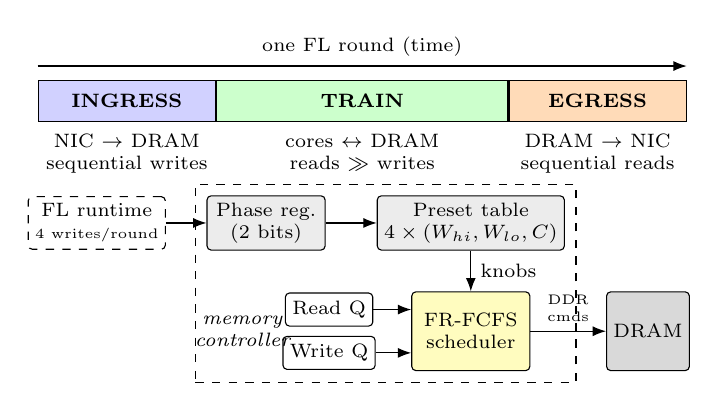
\begin{tikzpicture}[font=\scriptsize,>=Latex,
  ph/.style={draw,minimum height=0.52cm,inner sep=1pt},
  blk/.style={draw,rounded corners=1.5pt,minimum height=0.55cm,align=center,inner sep=2.5pt}]
% ---- round timeline
\node[ph,fill=blue!18,minimum width=2.25cm,anchor=west] (ing) at (-0.75,0) {\textbf{INGRESS}};
\node[ph,fill=green!20,minimum width=3.7cm,right=0pt of ing] (trn) {\textbf{TRAIN}};
\node[ph,fill=orange!28,minimum width=2.25cm,right=0pt of trn] (egr) {\textbf{EGRESS}};
\node[below=1pt of ing,align=center] (ingl) {NIC $\rightarrow$ DRAM\\sequential writes};
\node[below=1pt of trn,align=center] (trnl) {cores $\leftrightarrow$ DRAM\\reads $\gg$ writes};
\node[below=1pt of egr,align=center] (egrl) {DRAM $\rightarrow$ NIC\\sequential reads};
\draw[->] ([yshift=5pt]ing.north west) -- node[above,pos=0.5]{one FL round (time)} ([yshift=5pt]egr.north east);
% ---- controller
\node[blk,dashed,minimum width=1.45cm] (rt) at (0,-1.55) {FL runtime\\{\tiny 4 writes/round}};
\node[blk,fill=gray!15,minimum width=1.5cm] (reg) at (2.15,-1.55) {Phase reg.\\(2 bits)};
\node[blk,fill=gray!15,minimum width=2.3cm] (tab) at (4.75,-1.55) {Preset table\\$4\times(W_{hi},W_{lo},C)$};
\node[blk,minimum width=1.05cm,minimum height=0.42cm] (rq) at (2.95,-2.65) {Read Q};
\node[blk,minimum width=1.05cm,minimum height=0.42cm] (wq) at (2.95,-3.2) {Write Q};
\node[blk,fill=yellow!25,minimum width=1.5cm,minimum height=1.0cm] (sch) at (4.75,-2.925) {FR-FCFS\\scheduler};
\node[blk,fill=gray!30,minimum width=0.9cm,minimum height=1.0cm] (dram) at (7.0,-2.925) {DRAM};
\draw[->] (rt) -- (reg);
\draw[->] (reg) -- (tab);
\draw[->] (tab) -- node[right]{knobs} (sch);
\draw[->] (rq.east) -- (rq.east -| sch.west);
\draw[->] (wq.east) -- (wq.east -| sch.west);
\draw[->] (sch) -- node[above,font=\tiny,align=center]{DDR\\cmds} (dram);
\node[draw,dashed,inner sep=4pt,fit=(reg)(tab)(sch)(rq)(wq)] (mc) {};
\node[align=center,font=\scriptsize\itshape] at (1.85,-2.925) {memory\\controller};
\end{tikzpicture}
\caption{Top: memory traffic of one FL round on a client. Bottom: \name{}. The FL runtime writes the current phase; the phase selects the write-drain watermarks $W_{hi}$, $W_{lo}$ and the row-hit streak cap $C$ used by an otherwise unmodified FR-FCFS scheduler.}
\label{fig:overview}
\end{figure}

\section{\name{}}
\subsection{Phase Interface}
The controller holds a register $\textsc{phase}\in\{\textsc{idle},\textsc{ingress},\textsc{train},\textsc{egress}\}$. The FL runtime updates it through a privileged register write at the three points where the round changes character: before it starts receiving the model, before it starts local training, and before it starts sending the update; a fourth write returns it to \textsc{idle} at the end of the round.
% CHANGED: added the fourth (IDLE) write.
These points already exist as distinct calls in FL frameworks, so no application restructuring is needed. When the register holds \textsc{idle}, the controller behaves exactly as the baseline, so non-FL software is unaffected.

\subsection{Phase Presets}
\name{} does not introduce a new scheduling algorithm. It re-tunes three knobs that an FR-FCFS controller already has: the high and low write-queue watermarks $W_{hi}$ and $W_{lo}$, which decide when the controller enters and leaves write-drain mode, and the cap $C$ on consecutive row hits served before an older request to another row is considered. Table~\ref{tab:presets} lists the presets.

\begin{table}[t]
\centering
\caption{Phase presets of \name{}}
\label{tab:presets}
\footnotesize
\begin{tabular}{@{}llll@{}}
\toprule
Phase & Write drain & Row-hit cap $C$ & Intent \\
\midrule
\textsc{idle} & baseline & baseline & unchanged behaviour \\
\textsc{ingress} & eager: enter when & unlimited & long write bursts, \\
 & queue non-empty & & one activation per row \\
\textsc{train} & baseline $+$ age & baseline & no write backlog \\
 & bound $T_{max}$ & & blocks reads \\
\textsc{egress} & only at $W_{hi}$ & unlimited & uninterrupted \\
 & & & read stream \\
% CHANGED: TRAIN preset. The "lazy" rule (leave write mode as soon as a read arrives) was evaluated and was the
% worst variant (+0.3% round vs FR-FCFS; it adds turnarounds). The evaluated preset keeps the baseline
% watermarks and adds the T_max age bound (best: -1.13% round on the MLP client, robust for T_max 1000-8000).
% EGRESS cap: the baseline is FR-FCFS without a cap, so "raised" -> "unlimited". NOTE: the runs so far used
% cap 64 in EGRESS (no effect: egress is link-bound); set phasched_egress_cap = 1000000 for the final runs.
\bottomrule
\end{tabular}
\end{table}

\textbf{Ingress} favours writes. The controller enters write mode as soon as the write queue is non-empty and stays there until it is empty. Because the DMA stream fills rows in order, lifting the row-hit cap lets each row be activated once and written completely, and the number of write-to-read turnarounds falls to nearly zero.

\textbf{Train} keeps the baseline watermarks, so gradient and weight writes are drained in batches, but bounds their age: a write that has waited longer than $T_{max}$ triggers a drain. This prevents a backlog of write-backs from later blocking the reads in a long burst. Leaving write mode as soon as a read arrives performed worse, because it splits the drain into many short bursts that each pay a turnaround. The cap stays at its baseline value.
% CHANGED: TRAIN description rewritten to match the evaluated preset (see Table I comment).

\textbf{Egress} pins the controller in read mode without a row-hit cap,
% CHANGED: "with a raised cap" -> "without a row-hit cap".
 so the sequential read stream of the NIC is served in long row-hit runs; residual writes are drained only at $W_{hi}$.

\textbf{Starvation guard.} In every FL phase a request that has waited longer than $T_{max}$ is served next, and the controller switches to its queue if needed. This bounds the delay of any traffic that does not match the announced phase, such as a co-running application. We use $T_{max}=2000$ DRAM cycles (1.7\,$\mu$s).
% CHANGED: "every phase" -> "every FL phase" (IDLE stays exactly the baseline); added the queue switch and the
% T_max value. Measured: with the NIC saturating DRAM, FR-FCFS and BLISS delay co-running reads by ~231 us;
% the guard bounds this to ~1.7 us.

\subsection{Cost}
\name{} adds a 2-bit register, a four-entry table of watermark and cap values, and multiplexers on three existing comparators: fewer than 100 bits of state. Unlike ATLAS, TCM or BLISS it keeps no per-thread counters and performs no ranking.

\section{Evaluation Methodology}
We implement \name{} in DAMOV-SIM~\cite{damov}, which couples ZSim~\cite{zsim} with Ramulator~\cite{ramulator}. \emph{Network model:} DAMOV-SIM has no NIC. We add a DMA injector at the ZSim--Ramulator boundary that issues cache-bypassing write (ingress) and read (egress) requests over the model buffer at the configured link rate. \emph{Phase interface:} a ZSim magic instruction forwards the phase to the Ramulator controller. We enable DAMOV-SIM's memory-clock divider so that DDR4-2400 runs at 1.2\,GHz against the 2.4\,GHz cores. \emph{Workloads:} DAMOV contains no FL client, so we implement five synthetic FedAvg clients in C++/OpenMP with real forward and backward passes on synthetic local data (256\,MB per client); all parameters are kept in one buffer that the DMA injector transfers. Each run simulates one round with $K$ local minibatches; ingress and egress times are taken from the DMA injector.
% CHANGED: added clock-divider fix, workload description and how round time is measured.
\emph{System and workloads:} Table~\ref{tab:config}. \emph{Baselines:} FCFS, FR-FCFS, FR-FCFS with row-hit cap, and BLISS. \emph{Metrics:} round time and its per-phase breakdown, average and tail read latency, number of read/write bus turnarounds, and DRAM energy.

\begin{table}[t]
\centering
\caption{Simulated configuration}
\label{tab:config}
\footnotesize
\begin{tabular}{@{}ll@{}}
\toprule
Cores & 4 $\times$ 4-wide out-of-order x86-64, 2.4\,GHz \\
Caches & 32\,kB L1, 256\,kB L2, 8\,MB shared L3 \\
Memory & DDR4-2400, 1 channel, 1 rank, 32-entry read/write queues \\
Network & 10\,GbE (1.25\,GB/s), modelled by the DMA injector \\
Workloads & FedAvg clients: logistic regression (LR) and \\
 & naive Bayes (NB), 38\,MB; MLP 1024-2048-2048-10, \\
 & 24\,MB; 2-layer LSTM / GRU (hidden 512), 14 / 11\,MB \\
Round & one round; $K$=64/128/2/1/1 minibatches of \\
 & 512/512/32/8/8 samples (LR/NB/MLP/LSTM/GRU) \\
\bottomrule
\end{tabular}
\end{table}

\section{Preliminary Results}
Fig.~\ref{fig:results} reports round time normalised to FR-FCFS. \name{} shortens the round by 0.3\% on average (geometric mean) and by up to 1.1\% (MLP), and is never slower than FR-FCFS. At 10\,GbE, ingress and egress are bounded by the link and take the same time under every scheduler; they account for 58--62\% of the LR and NB rounds, whose sparse updates leave little for the scheduler to improve (${\le}0.02\%$). The gain comes from training in the dense clients (MLP, LSTM, GRU), where average read latency falls by 1.0\% on average and by up to 2.8\% (GRU), and the median read latency of the MLP drops by 20\%. Scheduling matters on these clients: FCFS lengthens the round by 43\% on average. The row-hit cap costs 0.6\%, and BLISS lengthens the round by 1.0\%, confirming that thread-level fairness does not capture phase behaviour. DRAM energy, estimated from the DRAM command counts and DDR4 datasheet currents, falls by 0.3\% on average and by up to 1.2\% (MLP), from the shorter round and up to 11\% fewer row activations.
% FILLED 2026-11-25: energy PhaSched/FR-FCFS 0.9999/1.0001/0.9884/0.9979/0.9979 geo 0.9968; ACT ratio
%   0.9999/1.0002/0.8924/0.9783/0.9652. Model: phasched/scripts/energy.py (typical 4Gb x8 DDR4-2400 IDD values).
% FILLED 2026-11-25 from the 10 GbE matrix (round = DMA-in + TRAIN + DMA-out, CPU cycles, normalised to FR-FCFS):
%   FR-FCFS-Cap 0.9999/0.9999/1.0079/1.0120/1.0094 geo 1.0058; BLISS 1.0077/1.0044/1.0301/1.0042/1.0047 geo 1.0101;
%   PhaSched 0.9998/1.0000/0.9887/0.9984/0.9985 geo 0.9971; FCFS geo 1.4306.
%   TRAIN avg read latency PhaSched/FR-FCFS: 0.9993/0.9997/0.9807/0.9971/0.9717 geo 0.9896; MLP p50 75 -> 60.
% CHANGED: removed "Ingress and egress shrink by [A%] and [B%] because bus turnarounds drop by [T%]".
% Measured: NIC transfer time is identical for all schedulers at 10/100/1000 Gbps (DMA timestamps); NIC-only
% phases have almost no turnarounds. [A%], [B%], [T%] are therefore not reported.

\begin{figure}[t]
\centering
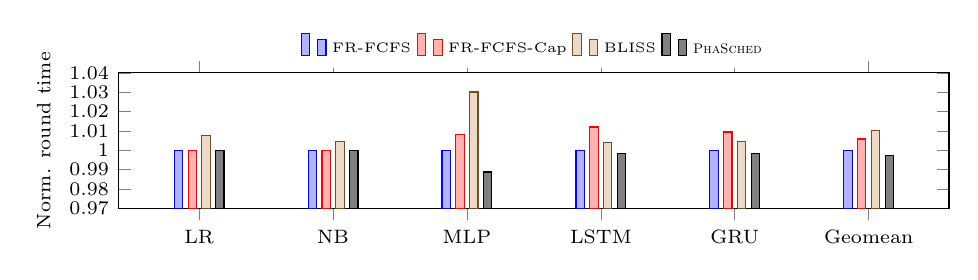
\begin{tikzpicture}
\begin{axis}[ybar,width=\columnwidth,height=3.3cm,ymin=0.97,ymax=1.04,ytick={0.97,0.98,0.99,1.00,1.01,1.02,1.03,1.04},yticklabel style={/pgf/number format/fixed,/pgf/number format/precision=2},
  ylabel={Norm. round time},ylabel style={font=\scriptsize},
  symbolic x coords={LR,NB,MLP,LSTM,GRU,Geomean},xtick=data,
  tick label style={font=\scriptsize},enlarge x limits=0.12,bar width=3pt,
  legend style={font=\tiny,at={(0.5,1.03)},anchor=south,legend columns=4,draw=none}]
% Measured values, normalised to FR-FCFS (10 GbE, one round).
\addplot coordinates {(LR,1) (NB,1) (MLP,1) (LSTM,1) (GRU,1) (Geomean,1)};
\addplot coordinates {(LR,0.9999) (NB,0.9999) (MLP,1.0079) (LSTM,1.0120) (GRU,1.0094) (Geomean,1.0058)};
\addplot coordinates {(LR,1.0077) (NB,1.0044) (MLP,1.0301) (LSTM,1.0042) (GRU,1.0047) (Geomean,1.0101)};
\addplot coordinates {(LR,0.9998) (NB,1.0000) (MLP,0.9887) (LSTM,0.9984) (GRU,0.9985) (Geomean,0.9971)};
\legend{FR-FCFS,FR-FCFS-Cap,BLISS,\name{}}
\end{axis}
\end{tikzpicture}
\caption{Round time normalised to FR-FCFS (lower is better; y-axis starts at 0.97).}
\label{fig:results}
\end{figure}

\section{Conclusion and Ongoing Work}
An FL round tells the system in advance what its memory traffic will look like. \name{} passes this knowledge to the memory controller with a 2-bit hint and re-tunes existing FR-FCFS knobs per phase. We are extending the study to asynchronous FL, where phases overlap, and to predicting the phase inside the controller from the read/write mix so that no software hint is required.

\bibliographystyle{IEEEtran}
\bibliography{refs}
\end{document}
